\documentclass{article}
\usepackage[utf8]{inputenc}

\usepackage{amsfonts}
\usepackage{enumitem}
\usepackage{amsmath}
\usepackage{xcolor}
\usepackage{hyperref}
\usepackage{graphicx}
\graphicspath{ {Figs/} }

\hypersetup{
    colorlinks=true,
    linkcolor=blue,
    filecolor=magenta,      
    urlcolor=cyan,
    pdftitle={Overleaf Example},
    pdfpagemode=FullScreen,
    }


\usepackage{geometry}
\geometry{margin=0.75in}



\begin{document}
\title{CMPSCI 389 Final Project Milestone 2 (HW6)}
\author{\textbf{Kamal Gurbanov, Graeme Reeves}}
\date{Assigned: April 23nd 2024; Due: April 30th 2024 @ 11:59 pm EST}

\maketitle

\begin{abstract}
    So now we're in the home stretch -- it's time for you to show off all of the work you've been pouring into your projects. Or it's time for you to scramble to get something together so that you manage to pass this class while also studying for finals. Either way, welcome to milestone 2! \\ \\
    \textbf{The final demos will be in class on May 15th}, so I hope this keeps you on track for that. You'll also need to put together a video demo for it by May 17th so get ready for that too! BTW, you should submit these in your groups, so hope you don't hate them yet!
    
\end{abstract}

\section{New results (35 points)}

Now that you know exactly what your final project is you have a whole extra week to get some new results. Just like last time, I want you to show some graphs/images of you progress. You can include whatever you have done (not code), but I expect 3 \textit{different} images that are higher quality than last time (label your axes and graph!). This homework doesn't have much you need to write, this is to give you time to produce some good stuff here, so use that time!


\begin{figure}[htb]
    \centering
    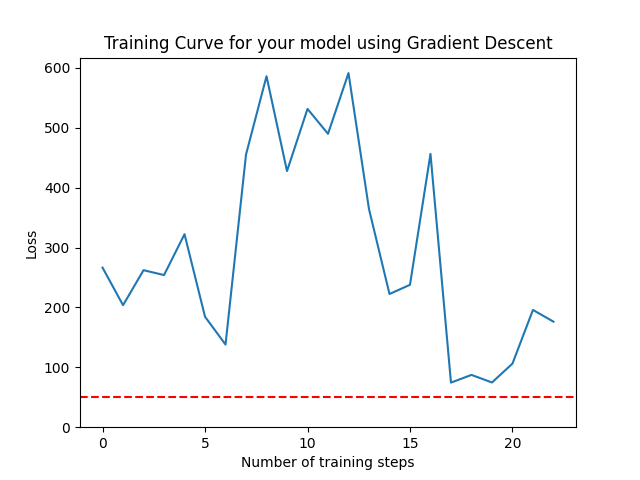
\includegraphics[width=0.4\textwidth]{Figs/Example training.png}
    \caption{ Example caption}
    \label{fig:net}
\end{figure}

\section{Result explanation (20 points)}

Here I want you to give detailed explanations of how you produced each graph and what the results of each mean. The results don't necessarily have to be good (though that's better) but the explanation has to be! You can combine this and the previous section so that the explanations go with the images if that is natural for you.


\section{Plan for Demos (25 points)}

You'll have to both give a demo in class and make a demo video of your project. In this section I want you to plan out both of these. Please include how each demonstration will work, what you'll show, and write a short synopsis of your explanation (the motivation, model setup, dataset used, etc ). Please do this part as a team!

So demonstration will be given by me and my partner Graem, for class demonstration we will probably use my laptop and we will show our project in jupyter notebook opened from Pycharm IDE however, if we will have some spare time before the due date I would love to create a simple web interface for our song recommendation engine, we will present our project by asking whoever is interested in or project their 5 favorite songs and 5 least favorite songs and input their names to the program and our model,hopefully!!!, will recommend the person song to listen. On top of that we already will have pre made examples for people to see who does not have time to think about the songs they like and do not like.

For the video part, me and my partner were thinking either create a small web interface to make our program seem a bit cooler and in a small video we would also include how we play song that was generated but I do not think we will write the code for that probably just generate from some player and also in that video we would make a 30 seconds explanation of the project. I promise, we will be very creative when we will be filming the video$)))$

\section{The bit where you can rant (15 points)} \textbf{Do this part after everything else.} In this part I want to hear what went well, what went okay and what didnt. List off 3 things that have gone well through this project so far, 3 things that you would do differently in hindsight. This is less important for me than it is for you -- I want you to be able to reflect that starting last minute or trying to invent AGI was a mistake.  

Well, one of the things that went well is finally, finding the right dataset for pre training, we had the problem of few-shot learning at first we were trying to only use 10 songs to train our model and obviously it failed because model was too dumb that's why we started to implement pre training model and for that we needed the actual dataset with labels 1,0 to implement supervised learning. Thank God we already found the dataset. Another thing that went well was API usage for pre training the model dataset we needed song lyrics and unfortunately spotify api does not provide us that, so we found Genius and song lyrics api that work and as I text right now it outputs all the song lyrics needed(probably will have more than a half a million songs.Another thing that went well is our subset construction at the end which works,we use faiss library to take all songs embedding and get the hypothetical song that user might like after user inputted his favorite songs and it would take that song and run it through our engine and it would output 1 if it thinks that user will like it and 0 otherwise.

3 things that I would do differently:

-I would research the topic more before starting programming, I did a lot of mistakes at the start connected to my lack of research and knowledge of the subject and I think i will do a bit more toward the end

-FIND THE RIGHT DATASET before I start programming, I did not know that finding,cleaning,formatting the dataset would be  one of the hardest challenges in my project

-Start early I think I only started working seriously on a project since this week and I only have 5 days to complete it and my pretraining model is not done yet, so in the future: classes, job and etc I will certainly try to start my ML projects mas early as possible.

\end{document}
